%!TEX root = ../main.tex

\subsection{Normal component}
\label{ss:normal_component}
\todo[inline]{Explain difference between fake and real normals.}
\todo[inline]{Explain structure of this section}
\begin{figure}
	\centering
	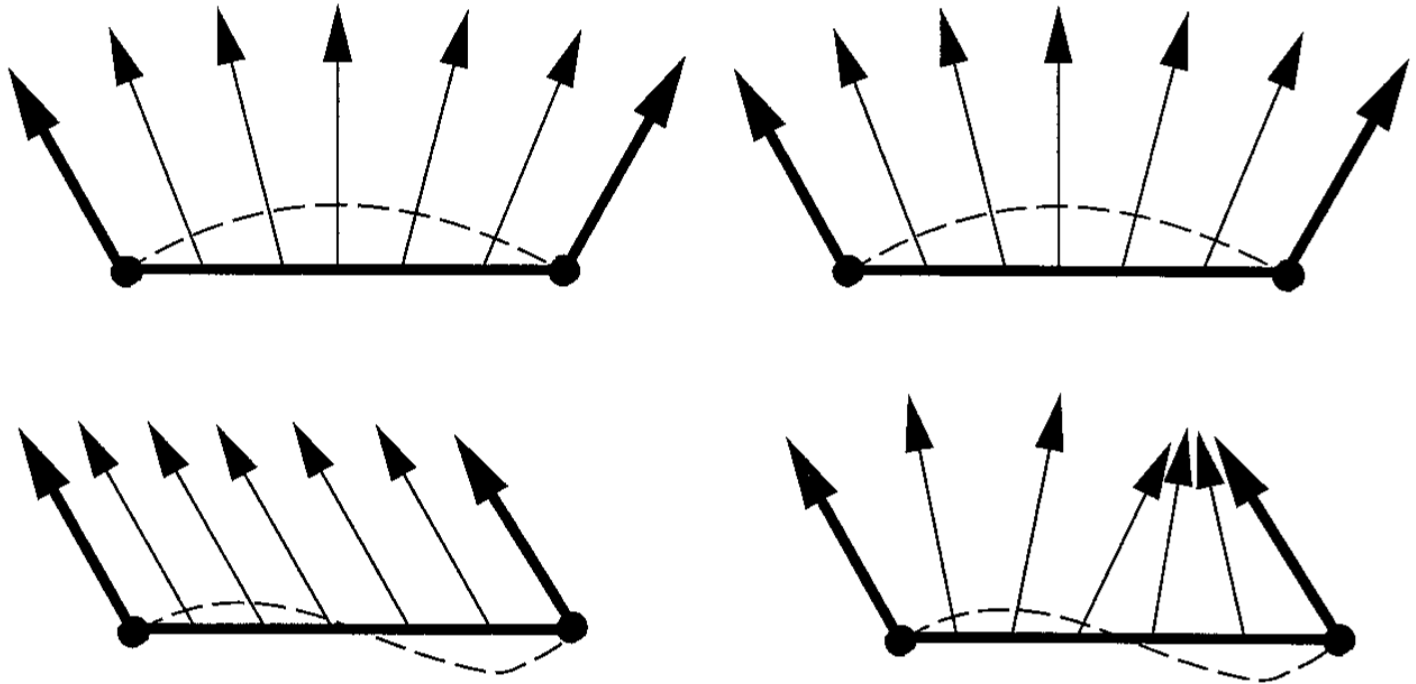
\includegraphics[width=0.48\textwidth]{./content/img/method/lin_vs_quad_varying_normals(inspiration).png}
	\caption{On the left: linear varying normals. On the right: quadratically varying normals. Illustration taken from \citeauthor{van1997phong}\textcite{van1997phong}. }
	\label{fig:3:linear_vs_quadratic_varying_normals}
\end{figure}

\subsubsection{Fake normals}
	\todo[inline]{We express normal component as a `quadratic' patch}
	\todo[inline]{Discuss parametrization of `quadratic' patch}
	\todo[inline]{Discuss the construction of the control points for the `quadratic' patch}

\subsubsection{Real normals}
	\todo[inline]{Discuss how to compute the real normals given the geometric component}